\documentclass[12pt]{exam}
\usepackage[utf8]{inputenc}

\usepackage[margin=1in]{geometry}
\usepackage{multicol}
\usepackage{enumitem}
\usepackage{amsmath, amscd, amssymb, amsthm, xspace, graphicx}
\usepackage{hyperref}
\usepackage[margin=1in]{geometry} % We can control the margins here
\usepackage[all]{xy}
\usepackage{subfigure}
\usepackage{float}
\usepackage{mathtools}  
\DeclarePairedDelimiter\Floor\lfloor\rfloor
\DeclarePairedDelimiter\Ceil\lceil\rceil

\newcommand{\class}{APPM 1350}
\newcommand{\term}{Fall 2021}
\newcommand{\examnum}{Quiz 2}
\newcommand{\examdate}{09/07/2021}
\newcommand{\timelimit}{10 Minutes}

\pagestyle{head}
\firstpageheader{}{}{}
\runningheader{\class}{\examnum\ - Page \thepage\ of \numpages}{\examdate}
\runningheadrule


\begin{document}

\noindent
\begin{tabular*}{\textwidth}{l @{\extracolsep{\fill}} r @{\extracolsep{6pt}} l}
	\textbf{\class} & \textbf{Name:} & \makebox[2in]{\hrulefill}\\
	\textbf{\term} &&\\
	\textbf{\examnum} &&\\
	\textbf{\examdate} &&\\
	\textbf{Time Limit: \timelimit} & Recitation Section: & \makebox[2in]{\hrulefill}
\end{tabular*}\\
\rule[2ex]{\textwidth}{2pt}

\begin{questions}

\question [7] Evaluate the limit 
$$\lim_{h \xrightarrow{} 0} \frac{\frac{1}{(4+h)^2}-\frac{1}{16}}{h}$$

\question From the following graph of the function f, calculate the following limits:
\begin{enumerate}[label=(\alph*)]
    \item (1 point) $\lim_{x \xrightarrow[]{} 2^-} f(x)$
    \item (2 points) $\lim_{x \xrightarrow[]{} 0} f(x)$. Make sure to explain your reasoning here. 
\end{enumerate}

\begin{figure}[H]
    \centering		
	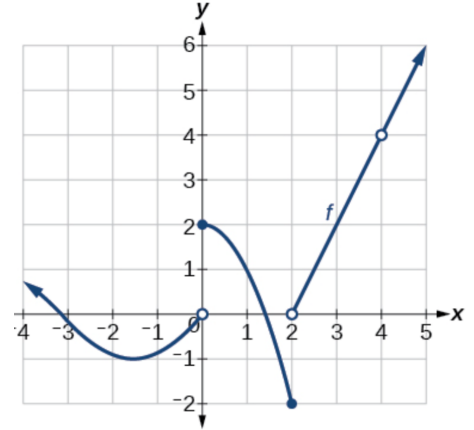
\includegraphics[width=.50\textwidth]{plot.png}
\end{figure} 

\end{questions}

\end{document}
